\chapter{Clientseitige Angriffe}

Client-seitige Angriffe zielen auf die Web-Browser der Benutzer ab und sind häufig Teil von Social Engineering Angriffen (da eine End-User Interaktion benötigt wird). Webserver besitzen die Möglichkeit, mittels optionaler HTTP Header den Clients Sicherheitspolicies und Verwendungshinweise mitzuteilen; Clients können auf diese Weise Schadcode erkennen und filtern.

\section{JavaScript-Injections (XSS)}
\index{xss}

Javascript-Injections (Cross-Site Scripting XSS) sind ein sehr häufig genutzter Angriffsvektor. Aufgrund der Häufigkeit dieses Angriffsvektor sind für diesen auch mehrere Hardening-Maßnahmen verfügbar.

Prinzipiell findet bei diesem Angriffsvektor der Angreifer einen Weg um JavaScript-Code innerhalb einer Webseite zu platzieren. Wird diese Webseite nun von einem Opfer in dessen Browser angezeigt, wird dieser Code exekutiert und der Angreifer kann auf diese Wiese unvorhergesehenen Code exekutieren.

Ein einfaches Beispiel wäre innerhalb der Kommentarfunktion einer Webseite möglich. Im Normalfall kann hier ein Benutzer Text eingeben, z.B. ``Hallo'', und dies wird für alle anderen Benutzer als Teil der HTML-Seite ausgegeben. Das resultierende HTML-Fragment könnte z. B. so aussehen:

\begin{minted}{html}
<div class="comment">
	<div class="author">Andreas Happe</div>
	<div class="content">Hallo</div>
</div>
\end{minted}

Ein Angreifer würde nun versuchen, JavaScript-Code als Eingabe zu übergeben, in der Hoffnung, dass dieser Code ungefiltert in der HTML-Ausgabe übernommen wird. Betrachtet ein anderer Benutzer nun diese Seite, würde dieser JavaScript-Code im Browser des anderen Benutzers ausgeführt werden. Ein einfaches Beispiel hierfür wäre die Eingabe von \textit{<script>alert(1);</script>}. Dieses JavaScript-Fragment ist relativ harmlos und öffnet nur ein Browser-Popup mit dem Text ``1''. Der resultierende HTML-Code (der im Browser des Opfers angezeigt werden würde) wäre:

\begin{minted}{html}
<div class="comment">
	<div class="author">Andreas Happe</div>
	<div class="content"><script>alert(1);</script></div>
</div>
\end{minted}

Ein Problem bei der defensiven Identifikation von potentiellen XSS-Lücken ist, dass die XSS-Angriffsfläche immens ist. Fast jede mögliche Benutzereingabe kann XSS-Schadmuster beinhalten. Ein Beispiel dafür wäre ein XSS-Fehler innerhalb von Flickr. Hier konnten Hacker XSS-Schadcode in den Metadaten der hochgeladenen JPEGs integrieren (z. B. als Kameramodel). Diese Daten wurden von Flickr ausgelesen, auf der Homepage ausgegeben und dadurch anderen Benutzern als Schadcode ``untergejubelt''. Ein weiteres Beispiel für unerwartete XSS-Angriffsvektoren ist dieses Dokument. Auf Anfrage hin habe ich eine eBook-Version dieses Dokuments erstellt und auf Amazon Kindle Direct Publishing hochgeladen. In der Entwurfsansicht wurden dann mehrere Hundert Rechtschreibfehler bemängelt. Wenn nun allerdings in der Detailansicht die Rechtschreibfehler betrachtet wurden, wurden automatisch XSS-Fragmente aus dem Dokument als Teil der Weboberfläche ausgeführt und hatten teilweise Zugriff auf Amazon-Cookies, etc.

\subsection{Arten und Payloads}

XSS-Angriffe werden in drei grobe Familien eingeteilt:

\begin{description}
	\item[Reflected XSS]\index{xss!reflected xss}: hier wird kein XSS-Code am Server persistiert sondern vom Server an den Client zurück reflektiert. Dies wird meistens durch das Einschleusen von JavaScript-Code über einen HTTP Parameter erfüllt --- dies impliziert allerdings auch, dass der Angreifer einen Weg findet, das Opfer zum Aufruf der modifizierten URL zu bewegen. Beispiel einer modifizierten URL: \url{http://opfer.xyz/operation?parameter=<script>alert(1)</script>}.
	\item[Stored/Persistent XSS]\index{xss!persistent xss}: hier besitzt der Angreifer die Möglichkeit den Javascript-Code am Server zu persistieren, ihn z. B. als Datenbank-Inhalt oder über eine hochgeladene Datei zuzustellen. Das Opfer betrachtet nun eine Webseite und bekommt durch den Server das XSS-Fragment übertragen. Ein Beispiel wäre das Übertragen von \mintinline{html}{<script>alert(1)</script>} als Chatnachricht innerhalb einer Webseite.
	\item[DOM-based XSS]\index{xss!dom-based xss}: dieser Angriffsvektor betrifft vor allem client-seitige Javascript-Frameworks die Eingaben aus dem DOM\footnote{Das Document-Object-Model beschreibt eine Programmierschnittstelle welche HTML/XML-Daten als Baumstruktur darstellt. Mittels Javascript kann das DOM modifiziert werden um beispielsweise Elemente bzw. deren Attribute hinzuzufügen, entfernen oder zu modifizieren; Eventhandler zu setzen bzw. Events zu feuern; bzw. um CSS zu verändern.} des Browsers übernehmen. Der Angreifer versucht, Schadcode innerhalb des DOMs zu platzieren (z. B. über die verwendete URL) und hofft, dass die Webapplikation dieses Element zum Bau einer Webseite verwendet. Bei dieser Form des XSS wird der bösartige Javascript Code erst im Client gebaut.
	\item[mXSS]\index{xss!mxss}: Webbrowser erlauben es, über eine Stringzuweisung in das \textit{innerHTML}-Attribute HTML-Code zu erstellen. Bevor der übergebene String in HTML-Code verwandelt wird, wenden die unterschiedlichen Browser-Familien Optimierungen (Mutationen) auf den String an. Dies kann ein Angreifer ausnutzen, indem er Schadcode so formatiert, dass er innerhalb des Strings noch harmlos wirkt, aber nach der String-Mutation bösartig wird.
	\item[uXSS]\index{xss!uxss}: Universal XSS zielen auf Fehler innerhalb von Webbrowsern bzw. innerhalb von Webbrowserplugin ab. Da diese auf ein Client-Programm abzielen, sind sie für diese Vorlesung out-of-scope.
\end{description}

Ein Problem an XSS-Angriffsmustern ist, dass diese sehr stark variieren können und daher schwer zu filtern sind; anbei mehrere XSS-Muster:

\begin{minted}{html}
<script>alert(1);</script>
<SCRIPT SRC=http://xss.rocks/xss.js></SCRIPT>

<IMG SRC=JaVaScRiPt:alert('XSS')>
<IMG SRC=`javascript:alert("RSnake says, 'XSS'")`>

<IMG SRC=javascript:alert(String.fromCharCode(88,83,83))>

<IMG SRC= onmouseover="alert('xxs')">
<IMG SRC="jav    ascript:alert('XSS');">
<BGSOUND SRC="javascript:alert('XSS');">
<IMG STYLE="xss:expr/*XSS*/ession(alert('XSS'))">
\end{minted}

Eine gute Quelle für weitere XSS-Beispiele ist das OWASP XSS Filter Evasion Cheat Sheet\footnote{\url{https://www.owasp.org/index.php/XSS_Filter_Evasion_Cheat_Sheet}}.

Mittels des eingeschleusten JavaScript-Code versucht der Angreifer nun, negativen Einfluss auf einen Benutzer zu nehmen. Ein gutes Beispiel wäre der Versuch, das Session-Cookie des aktuellen Benutzers (des Opfers) auszulesen und an einen externen Server zu übermitteln. Auf diese Weise würde ein Identitätsdiebstal durchgeführt werden. Ein weiteres Beispiel wäre \textit{Virtual Defacement}: bei diesem wird mittels JavaScript die dargestellt Webseite verändert und dadurch ein Defacement durchgeführt. Bösartig an diesem ist, dass die direkten Inhalte (Webseiten im Filesystem des Webservers) korrekt aussehen. In den letzten Jahren wurden XSS-Injections auch für Bitcoin/Crypto-Mining missbraucht. In diesem Fall wird jedes Opfer welches eine Webseite besucht kurzfristig Teil des Mining-Kollektivs. Last but not least kann XSS verwendet werden, um den Browser des Opfers Teil eines DDoS-Botnets zu machen. Ein berühmtes Beispiel hierfür ist die Low-Orbit Ion Canon die z. B. auch gerne von Anonymous verwendet wurde.

\subsubsection{Stehlen von Daten aus einem Passwortmanager}

Die meisten modernen Webbrowser bieten eine Form eines Passwortmanagers an. Nach einem durchgeführtem Login werden bei einem erneuten Besuch der Seite die Login-Credentials automatisch vom Webbrowser in das Formular eingetragen.

Falls ein Angreifer eine XSS-Lücke innerhalb eines Login-Formulars findet, kann er diese ausnutzen um die Login-Daten zu stehlen:

\begin{minted}{javascript}
<script>
document.write('<form><input id=password type=password style=visibility:hidden></form>');
setTimeout('alert("Password: " + document.getElementById("password").value)', 100);
</script>
\end{minted}

\subsection{Upload von HTML/Javascript-Dateien}
\label{upload_js}

Falls der Angreifer die Möglichkeit besitzt Dateien hochzuladen, kann dieser versuchen, auf diese Weise Javascript-Code in der Applikation zu hinterlegen. Hier ist der Angriffsvektor, diese Dateien von einem anderen Benutzer öffnen zu lassen. Da die hochgeladenen Dateien innerhalb der Applikation geöffnet werden, erhalten diese Zugriff auf sensible Benutzerdaten wie z. B. Session-Daten.

Auch hier sollten die erlaubten Dateitypen durch eine whitelist eingeschränkt werden. Zusätzlich sollte der \textit{Content-Disposition}-Header verwendet werden. Durch diesen teilt der Webserver dem Browser mit, dass eine Datei zum Download bestimmt ist. In diesem Fall lädt der Webbrowser die Datei herunter und öffnet anschließend potentiell die lokal heruntergeladene Datei --- dadurch ist diese nicht mehr Teil der Webapplikation und kann daher nicht mehr auf z. B. Session-Cookies zugreifen.

\subsubsection{X-Content-Type-Options}
\label{x_content_type_options}

Webserver übermitteln den MIME-Datentypen von übertragenen Dateien über den \textit{Content-Type} Header. Da diese Header ``früher'' ab und zu falsch gesetzt wurden, verwenden einige Browser (primär verschiedene Microsoft Internet Explorer und Edge Versionen) eine Heuristik um dynamisch den Content-Type zu bestimmen. Dabei wird der Anfang einer Datei gelesen, engl. ``sniffing'', und basierend auf der gefundenen Struktur ein MIME-Typ zugeordnet.

Dies kann ein Angreifer missbrauchen indem er z. B. ein Textfile hoch lädt (Datentyp \textit{text/plain}). Diese Datei enthält HTML-Code inklusive bösartigem JavaScript. Wenn nun ein Opfer auf dieses File zugreift und dessen Browser eine Heuristik verwendet, würde der Dateityp als JavaScript erkannt, und vom Browser das inkludierte bösartige JavaScript ausgeführt werden. Auf diese Weise kann der Angreifer eine potentielle Javascript-Upload-Sperre umgehen.

Mittels des \textit{X-Content-Type-Options: nosniff}-Headers kann der Webserver dem Webbrowser mitteilen, dass kein sniffing durchgeführt, und dem vom Server übermittelten Content-Type vertraut werden kann.

Zusätzlich blockieren Browser requests auf JavaScript- bzw. CSS-Dateien falls hier nicht der richtige Content-Type gesetzt ist (\textit{text/css} bzw. \textit{javascript}).


\subsection{Gegenmaßnahmen}

Gegenüber XSS-Angriffen werden prinzipiell zwei Gegenmaßnahmen empfohlen: Input Sanitation und Escaping von Ausgaben.

\subsubsection{Filtern der Eingaben}

Werden Daten aus nicht-vertrauenswürdigen Quellen verwendet, müssen diese automatisiert auf Schadmuster hin überprüft werden. Achtung: jegliche Form von Daten, die durch einen Benutzer bereitgestellt werden, sind automatisch nicht-vertrauenswürdige Daten. Ebenso muss beachtet werden, dass dies auch für Daten aus Benutzerhand gilt, die indirekt über eine Datenbank ausgelesen werden.

Da es eine Vielzahl möglicher Schadcodevarianten als auch viele potentielle Tarnmethoden gibt, ist das Filtern von Schadcode effektiv nur durch Verwendung einer (extern) gewarteten Bibliothek möglich.

Eine weiter Möglichkeit ist die Verwendung einer Web-Application Firewall wie z. B. \textit{mod\_security} im Zusammenspiel mit dem OWASP Core Rule Set (2). Hierbei wird jeder eingehende HTTP Request auf Schadcode hin überprüft und ggf. der Schadcode gefiltert bzw. der gesamte Request verworfen. Ein Problem bei der Verwendung von WAFs ist deren Ressourcen-Verbrauch als auch die potentiell hohe Anzahl von False-Positives (Anfragen die zwar nicht bösartig sind, aber von der WAF als bösartig erkannt, und daher geblockt werden).

\subsubsection{Quoting während der Ausgabe}

Um einen XSS-Angriff erfolgreich durchzuführen, muss der Javascript-Schadcode im Webbrowser des Opfers ausgeführt werden. Um dies bewerkstelligen zu können, muss eine bösartige Benutzereingabe Teil der dargestellten Webseite werden. Eine weitere Gegenmaßnahme gegenüber ist es daher, Benutzereingaben vor der Ausgabe so zu maskieren/quoten, dass diese nicht als Schadcode ausgeführt werden können. Dies wird häufig automatisiert durch Frameworks bzw. Bibliotheken durchgeführt.

Ein Problem dabei ist, dass die bösartige Benutzereingabe in Abhängigkeit der Verwendung unterschiedliche gequotet werden muss. Wird eine Eingabe als Teil einer URL verwendet, muss diese URL gequotete werden; wird eine Eingabe Teil von HTML muss diese HTML-gequoted werden. Wird eine Eingabe serverseitig als Teil von HTML ausgegeben und ist wiederum selbst Teil eines JavaScripts, dann muss die Eingabe sowohl Javascript- als auch HTML-gequotet werden. Eine gute Übersicht über diese Problematik gibt das OWASP XSS Prevention Cheat Sheet\footnote{\url{https://github.com/OWASP/CheatSheetSeries/blob/master/cheatsheets/DOM_based_XSS_Prevention_Cheat_Sheet.md}}. Ein einfaches Beispiel hierfür wäre folgendes serverseitige Source Code Fragment:

\begin{minted}{html}
<script>
var x = '<%= taintedVar %>';
var d = document.createElement('div');
d.innerHTML = x;
document.body.appendChild(d);
</script>
\end{minted}

Die Variable \textit{taintedVar} wird hier in einen Javascript-String eingefügt (Zeile 2), hierbei muss sie gequoted werden, damit Schadcode nicht den String schließen und bösartigen Javascript-Code exekutieren würde. Zusätzlich wird die Eingabe zum Wert der Variable \textit{x} und dieser Wert wird in die HTML Seite eingebaut. Dadurch wird diese Variable als HTML-Code interpretiert und auch auf diese Weise könnte bösartiger Code eingebaut werden.

Einige Grundregeln zur Verwendung von user-supplied Daten innerhalb von Javascript:

\begin{itemize}
\item Die Verwendung von Benutzerdaten sollte so weit wie möglich minimiert werden.
\item User-Supplied Daten sollten niemals auf der linken Seite (LHS) einer Zuweisung verwendet werden.
\item die Methoden \textit{element.write} und \textit{element.writeln} als auch die Attribute \textit{innerHTML} und \textit{outerHTML} rendern die übergebenen Texte als HTML-Code. Dabei kann auch Code exekutiert werden --- es wird empfohlen stattdessen \textit{innerText} und \textit{textContent} zu verwenden.
\item die Methode \textit{eval} sollte vermieden werden. Achtung: teilweise wird eval intern verwendet (z. B. bei Verwendung von Timeout-Funktionen), hier sollten keine Benutzereingaben verwendet werden.
\item Ebenso sollte niemals user-supplied Data als Event-Handler verwendet werden.
\end{itemize}

\subsection{Hardening mittels X-XSS-Protection}
\label{x_xss_protection}

Moderne Browser verwendeten Heuristiken um \textit{Reflected-XSS} Angriffe automatisiert zu erkennen. Zumeist werden hierfür die ausgehenden HTTP Requests (inkl. Parameter) mit den eingehenden Antwortdokumenten verglichen.

Leider kann nicht davon ausgegangen werden, dass bei Browsern diese Heuristik per Default aktiviert oder deaktiviert ist --- das Verhalten kann allerdings mittels des \textit{X-XSS-Protection}-Header gesteuert werden. Es wird daher empfohlen, diesen Header zu setzen um undefiniertes Verhalten zu vermeiden.

Folgende Werte sind für den Header erlaubt:

\begin{itemize}
	\item \textbf{0}: die XSS-Heuristik soll deaktiviert werden.
	\item \textbf{1}: die XSS-Heuristik soll aktiviert werden, erkannte potentielle XSS-Schadmuster werden aus der Ausgabe entfernt.
	\item \textbf{1;mode=block}: die XSS-Heuristik soll aktiviert werden, falls XSS-Schadmuster erkannt werden wird keine Webseite gerendert.
\end{itemize}

Während das automatische Filtern von XSS-Schadcode theoretisch positiv aus Sicherheitssicht sein sollte, war dies in der Praxis fehlerbehaftet und führte zu folgenden Problemen:

\begin{itemize}
	\item False-Positives: nicht bösartiger Schadcode wurde als Schadcode erkannt und gefiltert. Dadurch wurde die Funktionsfähigkeit korrekt programmierter Webseiten eingeschränkt.
	\item Wird X-XSS-Protection im Default-Modus verwendet, versucht der Browser nur den Schadcode aus dem Antwortdokument zu filtern. Dies kann gezielt durch Angreifer ausgenutzt werden, um auf diese Weise XSS-Code zu generieren\footnote{Dies wird als UXSS bezeichnet, siehe auch \url{https://blog.innerht.ml/the-misunderstood-x-xss-protection/}.}.
\end{itemize}

Aus diesem Grund ignorieren moderne Browser diesen Sicherheitsheader mittlerweile (Google Chrome, Mozilla Firefox und Microsoft Edge, Stand 31.12.2019). Als Gegenmaßnahme gegenüber XSS kann daher nur der Einsatz von CSP empfohlen werden (abgesehen davon, XSS-Lücken generell nicht zu implementieren).

\subsection{Hardening mittels CSP}

Die Content Security Policy kann verwendet werden um potentielle Javascript-Lücken zu vermeiden. Hierbei wird durch eine Policy definiert in welchen Dateien überhaupt Javascript-Code vorkommen darf. Falls eine saubere Trennung in JavaScript- und HTML-Dateien durchgeführt wurde, kann die Definition von JavaScript-Fragmenten in HTML Dateien vollkommen deaktiviert werden. Falls es ein Angreifer nun schafft, durch eine Injection Lücke JavaScript-Code in einer HTML-Seite zu platzieren, würde dieser durch den Browser einfach ignoriert werden.

Ein Problem beim Einsatz von CSP sind \textit{polyglot} Files. Dies sind Dateien, die so gebaut wurden, dass sie gleichzeitig zwei unterschiedliche Datentypen erfüllen. Ein Beispiel für ein polyglot File ist eine JPEG-Datei welche, wenn sie als Textdatei eingebunden wird, validen Javascript-Code beinhaltet. Ein Beispiel für solche Dateien kann unter \url{https://portswigger.net/blog/bypassing-csp-using-polyglot-jpegs} gefunden werden. Dies ist problematisch, da ein Angreifer ein JavaScript File als Bild hochladen kann (während der Upload von JavaScript-Files normalerweise durch eine Webapplikation blockiert wird) und danach mittels eines \textit{script}-Tags dieses Bild als Javascript-Source File innerhalb von HTML inkludieren kann. Dies umgeht potentielle CSP-Richtlinien.

\section{CSRF Angriffe}

CSRF-Angriffe nutzen ein bestehendes Vertrauensverhältnis zwischen dem Web-Browser des Opfers und einem Webserver aus. Das grundsätzliche Problem ist, das Webbrowser, bei Requests zu bereits eingeloggten Webservern, automatisch Sessions anhängen. Dabei wird nicht überprüft, ob der ausgehende Request wirklich vom Benutzer in Auftrag gegeben worden ist.

Folgende Schritte würden bei einem typischen CSRF-Szenario passieren:

\begin{enumerate}
\item Der Benutzer (im Folgenden das Opfer genannt) loggt sich bei einem Webserver ein. Der Webbrowser des Benutzers speichert sich das Session-Cookie für Folgezugriffe auf diesen Webserver.
\item Der Benutzer surft im Internet und besucht dabei einen durch den Angreifer kontrollierten Webserver.
\item Auf diesem Webserver befindet sich ein Formular, welches eine Operation auf dem Webserver, auf dem das Opfer eingeloggt ist, aufruft.
\item Der Browser des Opfers lädt die Webseite vom Webserver des Angreifers. Das Formular wird entweder durch den unbedarften Anwender oder durch Javascript automatisch abgesendet.
\item Der Browser des Opfers hängt automatisch das Session-Cookie zu dem ausgehenden Request hinzu.
\item Der Webserver (auf dem das Opfer eingeloggt war) erhält nun einen Request mit einer validen Session ausgehend vom Webbrowser des Opfers. Da dieser Request vollkommen korrekt aussieht, wird dieser auch exekutiert.
\end{enumerate}

Ein Beispiel für ein HTML Formular welches der Angreifer auf seinem Webserver hinterlegen würden:

\begin{minted}{html}
<form action="http://bank.com/transfer.do" method="POST">
<input type="hidden" name="acct" value="MARIA"/>
<input type="hidden" name="amount" value="100000"/>
<input type="submit" value="View my pictures"/>
</form>
\end{minted}

\begin{figure}
	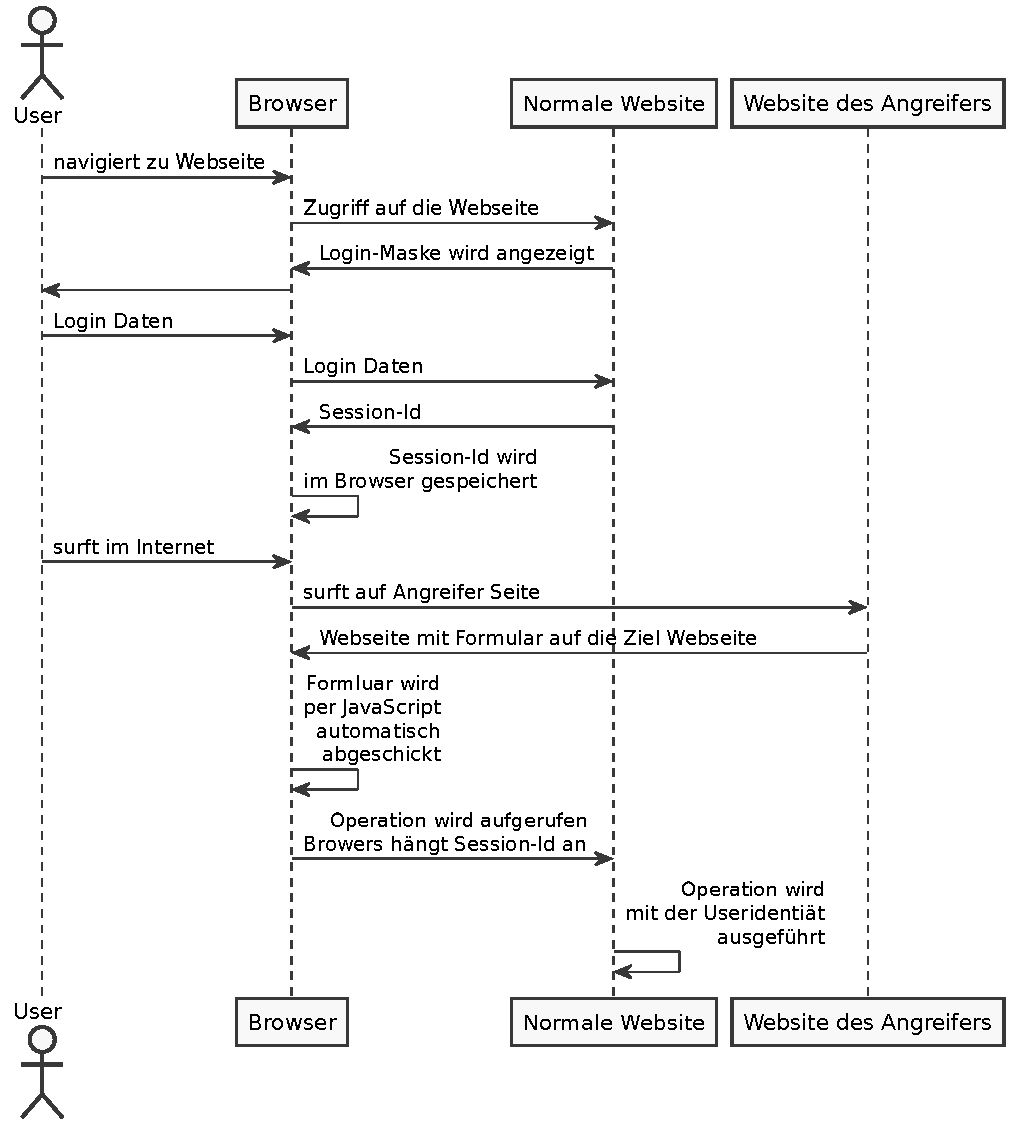
\includegraphics[width=\textwidth]{graphs/csrf.pdf}
	\centering
	\caption{Beispiel für einen CSRF-Angriff}
\end{figure}

In diesem Fall wird die Operation \url{http://bank.com/transfer.do} mit den Parametern \textit{acct} und \textit{amount} aufgerufen. Bei diesem Beispiel wurden die Felder versteckt und der Button mit einem \textit{ablenkenden} Text beschriftet. Alternativ könnte der Angreifer das Formular auch in einem 1x1 Pixel großem IFrame verstecken und automatisiert mittels Javascript abschicken.

\subsection{Synchronizer Token Pattern}

Es gibt mehrere Gegenmaßnahmen gegen CSRF-basierte Angriffe, sicherheitstechnisch ist das so genannte \textit{Synchronizer Token}-Pattern vorzuziehen. Bei diesem fügt der Webserver bei jedem Formular ein verstecktes HTML-Feld hinzu, in dieses schreibt der Server einen zufälligen Zahlenwert. Wird eine Operation am Server aufgerufen wird dieses Feld an den Server übertragen und dieser vergleicht den übertragenen Zahlenwert mit dem vom Server erwarteten Zahlenwert. Falls diese übereinstimmen, wird die Operation ausgeführt, ansonsten wird die Operation verworfen. Dieser Schutz funktioniert, da der Angreifer auf seinem remote Server den Zahlenwert erraten und in das Angriffs-Formular einfügen müsste.

Damit dieser Schutz verlässlich funktioniert, muss der Zahlenwert regelmäßig erneuert werden, bevorzugterweise sollte für jede potentielle Operation ein neuer Zufallswert generiert werden. In der Praxis wird diese Anti-CSRF Maßnahme häufig vollkommen transparent und automatisch durch das verwendete Web-Framework implementiert.

Wichtig ist, dass eine Operation die einen CSRF-Check implementiert nicht nur überprüft, ob ein potentiell übergebener CSRF-Wert mit dem server-gespeicherten CSRF-Wert übereinstimmt, sondern auch überprüft ob überhaupt ein CSRF-Wert übergeben wurde. Während Tests wurde häufig das fehlerhafte Verhalten vorgefunden, dass wenn der CSRF-Parameter einfach gelöscht wird, die Operation ausgeführt wird (also CSRF-Tokens nur verglichen werden, wenn beim Aufruf zumindest ein CSRF-Wert übergeben wird).

\subsection{SameSite-Flag bei Session Cookies}

Eine weitere Schutzmaßnahme (im Sinne des Hardening) ist der Einsatz des \textit{SameSite} Cookie-Flags (siehe auch Kapitel \ref{session_cookies_samesite}, Seite \pageref{session_cookies_samesite}). Bei korrektem Setzen dieses Flags erlaubt der Web-Browser des Opfers das Übertragen der Session-Id nur, wenn sowohl das Formular als auch das Ziel des Formulars sich auf dem identen Webserver befinden.

\section{Unverified Forwards and Redirects}

Diese Schwachstelle war in den OWASP Top 10 2013 vorhanden, wurde allerdings 2017 aus der Liste der Top 10 entfernt. Die Schwachstelle entsteht, falls eine Operation einer Webapplikation den Benutzerbrowser auf eine weitere Seite weiterleitet und das Ziel über einen Parameter bestimmt wird. Ein Angreifer kann nun versuchen, das Opfer auf eine externe Seite zu leiten um dies im Zuge eines Social Engineering Angriffs auszunutzen. Eine verwundbare Operation würde z. B. folgendermaßen aussehen: \url{http://example.com/example.php?url=http://malicious.example.com}.

Besonders gefährlich ist es, wenn die verlinkte URL nicht über ein HTTP Redirect aufgerufen wird, sondern wenn die übergebene URL als Ziel eines eingebetteten IFrames verwendet wird. Auf diese Weise kann der Angreifer Inhalte auf der (vermeintlichen) Opferwebseite platzieren, die meisten Enduser werden nicht bemerken, dass sie gerade Daten in einem Iframe und nicht in der Opfer-Webseite eingeben.

Falls es wirklich notwendig sein sollte, dass eine Zieladresse über einen URL-Parameter übergeben wird, sollte penibles Whitelisting der erlaubten URLs betrieben werden.

\section{Clickjacking}

Clickjacking wird auch teilweise \textit{UI redress attack} genannt. Bei diesem Angriff will der Angreifer einen unbedarften Benutzer dazu bringen, eine Webseite zu bedienen. Um dies durchzuführen, baut der Angreifer eine eigene, harmlos aussehende, Webseite, welche den identen Bedienfluss wie die Webseite besitzt, die der Angreifer gerne fernsteuern würde. Mittels eines IFrames wird die Opferwebseite über die erstellte Webseite des Angreifers gelegt, die Transparenz der Opfer-Webseite wird auf 100\% gesetzt.

Wenn nun der Benutzer die vermeintliche (vom Angreifer erstellte) Webseite bedient, werden in Wirklichkeit alle Benutzereingaben an die transparente Opfer-Webseite übertragen und dadurch diese durch den Benutzer ferngesteuert.

Eine gute Abwehrmassnahme gegen Clickjacking ist der \textit{X-Frame-Options} HTTP Header.

\subsection{X-Frame-Options}
\label{x_frame_options}

Der \textit{X-Frame-Options} Header wird verwendet um dem Webbrowser mitzuteilen, innerhalb welcher Webseiten die eigene Webseite eingebunden werden darf. Dadurch werden Clickjacking-Angriffe unterbunden.

Der Webserver kann über das Setzen des \textit{X-Frame-Options} Header auf folgende Werte das Webbrowser-Verhaltensmuster beeinflussen:

\begin{description}
	\item[DENY]: die Webseite darf nicht von anderen Webseiten mittels IFrames eingebunden werden.
	\item[SAMEORIGIN]: die Webseite darf von allen Webseiten mit dem identen Origin eingebunden werden.
	\item[ALLOW-FROM domain]: die Webseite darf explizit von der Domain \textit{domain} eingebunden werden.
\end{description}

\section{Reverse Tab Nabbing}

Bei einem Reverse Tab Nabbing navigiert der Benutzer zuerst auf eine Opferseite. Diese öffnet nun einen Link auf eine bösartige Seite in einem neuen Fenster. Die aufgerufene bösartige Seite verwendet nun Javascript um die Adresse der aufrufenden Seite (die wahrscheinlich gerade im Hintergrund ist) zu verändern, der Webbrowser führt nun ein redirect auf die neu verlinkte Seite im Hintergrund vor (während der Benutzer noch immer die neu geöffnete Seite betrachtet). Wenn der Benutzer nun das geöffnete Fenster schließt befindet er sich vermeintlich auf der ursprünglichen Seite, welche den Link öffnete, befindet sich allerdings in Wirklichkeit auf einer Seite, die vom Angreifer bestimmt wurde.

Ein Beispiel für Reverse Tab Nabbing, folgende Opfer Seite:

\begin{minted}{html}
<html>
  <body>
    <li><a href="bad.example.com" target="_blank">Vulnerable target using html link to open the new page</a></li>
    <button onclick="window.open('https://bad.example.com')">Vulnerable target using javascript to open the new page</button>
  </body>
</html>
\end{minted}

Die Opferwebseite öffnet eine externe Seite über einen Link (mittels \textit{target=\_blank} wird ein neues Fenster geöffnet) bzw. alternativ über Javascript (\textit{onclick}). Als neue Webseite verwendet der Angreifer folgendes:

\begin{minted}{html}
<html>
  <body>
    <script>
      if (window.opener) {
        window.opener.location = "https://phish.example.com";
      }
    </script>
  </body>
</html>
\end{minted}

Der Angreifer setzt über \textit{window.opener} die Adresse der aufgerufenen Seite und ändert dadurch (im Hintergrund) die im Webbrowser dargestellte Seite. Wenn der Benutzer die geöffnete Seite schließt, gelangt er dadurch auf eine vom Angreifer modifizierte Webseite.

Als Gegenmaßnahme sollte bei ausgehenden Links immer das \textit{rel} Attribute auf \textit{noopener noreferrer} gesetzt werden. Dadurch kann die geöffnete Seite nicht mehr über \textit{windows.opener} auf die Location der öffnenden Seite zugreifen. Zusätzlich kann über die \textit{Referrer-Policy} das Übermitteln des Referrer-Headers an die aufgerufene Webseite unterbunden werden.

\textbf{Update 2020}: mehrere Browser bieten mittlerweile automatische Verteidigungsmassnahmen gegenüber Reverse Tabnabbing Angriffe. Firefox (seit 2016), Microsoft Edge und Firefox sollten out-of-the-box nicht mehr gegenüber diesem Angriff verwundbar sein (sie setzen das \textit{noopener}-Flag automatisch). In zukünftigen Google Chrome Versionen ab 2021 sollte diese Browserfamilie dies auch durchführen und auf diese Weise Tabnabbing-Angriffe unterbinden.

\section{HTML5 PostMessage als Angriffskanal}

Eine Webapplikation wird innerhalb eines Browser-Tabs geöffnet, ihre Einflussmöglichkeiten (z. B. mittels Javascript) beschränken sich auf Inhalte innerhalb des Browser-Tabs. Es gibt Use-Cases, bei denen eine Applikation mit einer Webseite innerhalb eines anderen Browser-Tabs bzw. Browser-Fensters interagieren will. Ein Beispiel sind web-basierte Präsentationsframeworks. Hier gibt es meistens zwei Browserfenster: eines für die aktuell dargestellte Präsentationsfolie und ein Fenster mit Notzien für den Vortragenden. Wird die Folie gewechselt sollten im zweiten Fenster ebenso die Kommentare für die aktuell angezeigte Folie dargestellt werden.

Eine moderne Implementierungsmöglichkeit für diese Funktion ist \textit{HTML5 postMessage}. Die Webseite, welche eine Aktion ausführen will, kann eine Nachricht via Javascript absenden. Diese Nachricht beinhaltet die message, einen \textit{Target-Origin} (kann auch das Wildcard \textit{*} sein) und eine Liste von serialisierten Objekten (deren Owernship an den Empfänger übergehen). Die empfangende Webseite kann einen Callback-Handler für empfangene Webseiten registrieren und auf diese Weise auf die Nachricht reagieren.

Ein Beispiel für einen Message-Handler:

\begin{minted}{html}
<script>
function messageHandler(event){
	from = "From: " + event.origin;
	data = "Data: " + event.data;
	alert(from);
	alert(data)
}
// Register the handler
window.addEventListener("message", messageHandler)
</script>
\end{minted}

Das Beispiel zeigt bereits eine Schwachstelle von HTML5 postMessage: der \textit{origin} wird nicht durch den Empfänger überprüft, sondern durch den Code des Empfängers.

Wie kann eine Nachricht gesendet werden?

\begin{minted}{html}
otherWindow.postMessage(message, targetOrigin, [transfer])
\end{minted}

Die jeweiligen Variablen wären:

\begin{itemize}
\item \textbf{otherWindow} gibt den Empfänger an. Dieser kann z. B. \textit{parent}, ein Iframe, \textit{window.opener} oder\textit{window.source} sein.
\item \textbf{message} ist der String der als Nachricht an den Empfänger übertragen wird.
\item \textbf{targetOrigin} gibt die origin des Empfängers an, kann aber auch als Wildcard (\textit{*}) ausgeführt sein.
\item \textbf{tranfer} ist eine Liste von übertragenen Objekten. Diese können vom Sender nicht mehr verwendet werden und gehen in den Besitz des Empfängers über.
\end{itemize}

Hier ergeben sich zwei Angriffsszenarien:

\begin{enumerate}
	\item Eine Webseite akzeptiert Nachrichten von beliebigen Quellen. Dies könnte z. B. im Zuge eines XSS-Angriffs ausgenutzt werden.
	\item Beim Senden der Nachricht werden sensible Daten versendet ohne dass der Empfänger eingeschränkt wird. Dies geht zumeist mit einer \textit{TargetOrigin} von \textit{*} herein.
\end{enumerate}

\section{Reflektionsfragen}

\begin{enumerate}
\item Erkläre Reflected-, Stored- und DOM-Based XSS Angriffe. Welche Gegenmaßnahmen gibt es und erläutere diese.
\item Was sind unvalidated Forwards und Redirects? Wie kann dagegen geschützt werden?
\item Was sind Reverse Tab Nabbing Angriffe? Welche Absicherungsmaßnahmen gibt es dagegen?
\item Welche Sicherheitsprobleme können bei HTML5 Local Storage auftreten?
\item Wie funktionieren Clickjacking-Angriffe und wie können diese verhindert werden?
\item Wie funktioniert ein CSRF-Angriff? Erläutere zwei potentielle Gegenmaßnahmen?
\end{enumerate}
